% !Mode:: "TeX:UTF-8"
\chapter{3D Rigid Body Motion}
\label{cpt:3}

\begin{mdframed}
	\textbf{Goal of Study}
	\begin{enumerate}
		\item Study the rigid body geometry in three-dimensional space: rotation matrix, transformation matrix, quaternion, and Euler angle.
		\item Learn the usage of the \textit{Eigen} library's matrix and geometry module.
	\end{enumerate}
\end{mdframed}

In the last lecture, we explained the framework and content of visual SLAM. This lecture will introduce one of the fundamental problems of visual SLAM: How to describe a rigid body's motion in three-dimensional space? Intuitively, we certainly know that this consists of one rotation plus one translation. The translation part does not really have any problems, but the rotation part is questionable. We will introduce the meaning of rotation matrices, quaternions, Euler angles and how they are computed and transformed. In the practice section, we will introduce one of the widely used linear algebra libraries: \textit{Eigen}. It provides a C++ matrix calculation, and its geometry module also provides the necessary data structures and operations, like quaternions. \textit{Eigen} is heavily optimized, but there are still some special issues to be discussed about its usage. We will leave it to the practice part.

\newpage
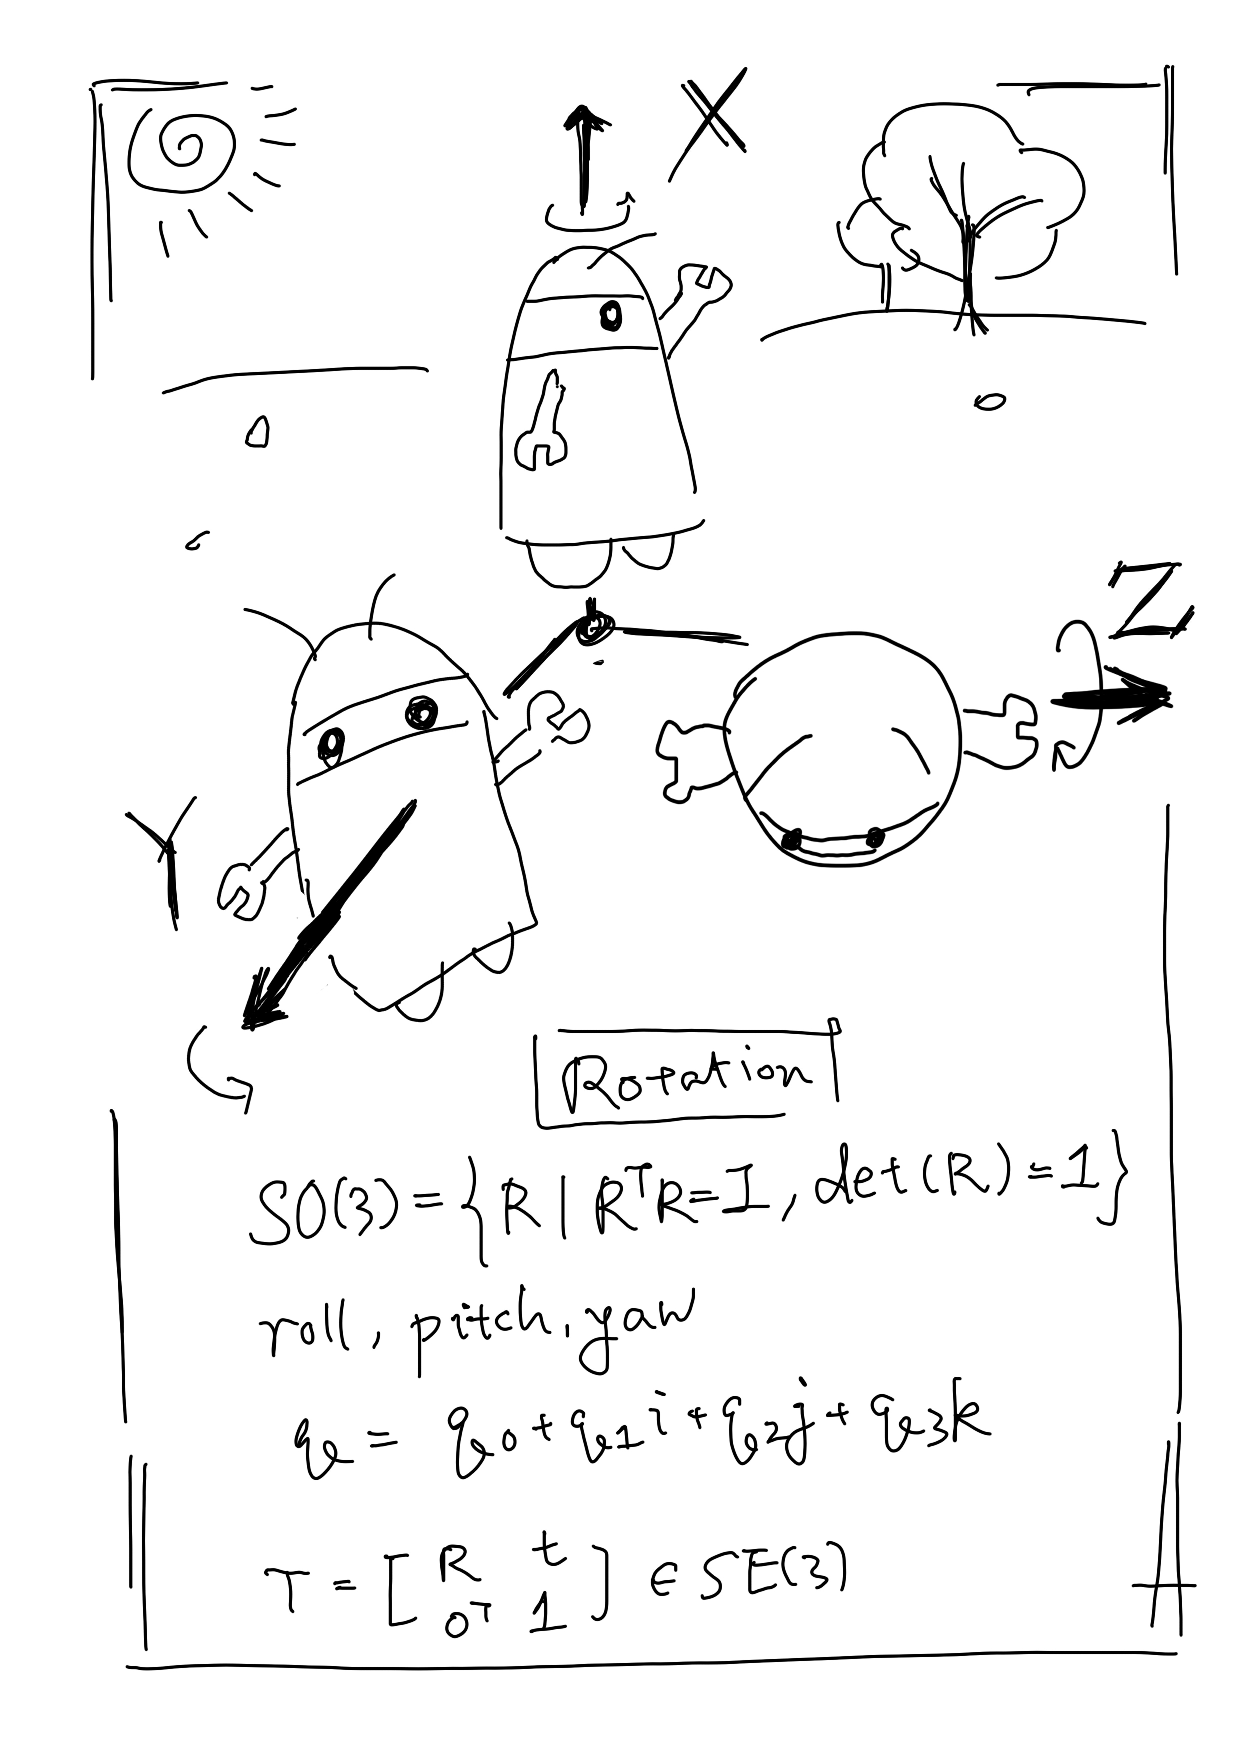
\includepdf{resources/other/ch3.pdf}
\newpage

\section{Rotation Matrix}
\label{sec:3.1}
\subsection{Points, Vectors, and Coordinate Systems}
The space of our daily life is three-dimensional, so we are born to be used to 3D movements. The 3D space consists of three axes, so the position of one spatial point can be specified by three coordinates. However, we should now consider a rigid body, which has its \textit{position} and \textit{orientation}. The camera can also be viewed as a rigid body in three dimensions, so what we care about in VSLAM are the problem of the camera's position and orientation.  Combined, we can say, ``the camera is at the $( 0, 0, 0)$ point, facing the front''. But this natural language is troublesome, and we prefer to describe it in a mathematical language.

We start from the most basic content: \textit{points} and \textit{vectors}. Points are the basic elements in space, no length, no volume. Connecting the two points forms a vector. A vector can be thought of as an arrow pointing from one point to another. Here we need to remind the reader that please do not confuse the vector with its coordinates. A vector is one thing in space, such as $ \mathbf{a}$. Here $ \mathbf{a} $ does not need to be associated with several real numbers. We can naturally talk about the plus or minus operation of two vectors, without relating to any real numbers. Only when we specify a coordinate system in this 3D space can we talk about the vector's coordinates in this system, finding several real numbers corresponding to this vector.

With the knowledge of linear algebra, the coordinates of a point in 3D space can be described by $ \mathbb{R}^3$. How to describe it? Suppose that in this linear space, we find a set of base \footnote{Just a reminder here, the base is a set of linearly independent vectors in the space, normally being orthogonal and has unit-length.} $ (\mathbf{e}_1,\mathbf{e}_2,\mathbf{e}_3) $, then, an arbitrary vector $ \mathbf{a} $ has a \textit{coordinate} under this base:
\begin{equation}
\mathbf{a} = \left[ {{\mathbf{e}_1},{\mathbf{e}_2},{\mathbf{e}_3}} \right]\left[ \begin{array}{l}
{a_1}\\
{a_2}\\
{a_3}
\end{array} \right] = {a_1}{\mathbf{e}_1} + {a_2}{\mathbf{e}_2} + {a_3}{\mathbf{e}_3}.
\end{equation}

Here $ (a_ 1, a_ 2, a_ 3 )^{T} $ is called $\mathbf {a}$'s coordinates \footnote {We use column vectors in this book which is same as most of the  mathematics books.}. The coordinates' specific values are related to the vector itself and the selection of the bases. In $\mathbb{R}^3$, the coordinate system usually consists of 3 orthogonal coordinate axes (it can also be non-orthogonal, but it is rare in practice). For example, given $ \mathbf {x} $ and $ \mathbf {y} $ axis, the $ \mathbf {z} $ axis can be determined using the right-hand (or left-hand) rule by $ \mathbf {x} \times  \mathbf {y} $. According to different definitions, the coordinate system is divided into left-handed and right-handed. The third axis of the left-hand rule is opposite to the right-hand rule. Most 3D libraries use right-handed coordinates (such as OpenGL, 3DS Max, etc.), and some libraries use left-handed coordinates (such as Unity, Direct3D, etc.).

Based on basic linear algebra knowledge, we can talk about the operations between vectors/vectors, vectors/numbers, such as scalar multiplication, vector addition, subtraction, inner product, outer product, and so on. Multiplication, addition, and subtraction are fairly basic and intuitive. For example, the result of adding two vectors is to add their respective coordinates, and the same for subtraction, and so on. I won't go into details here. Inner and outer products may be somewhat unfamiliar to the reader, and their calculations are given here. For $ \mathbf {a}, \mathbf {b} \in  \mathbb {R}^ 3 $, in the common definition \footnote {The inner product also has more general definitions, but this book only discusses the usual inner product.}, the inner product of $\mathbf{a}, \mathbf{b}$ can be written as:

\begin{equation}
\mathbf{a} \cdot \mathbf{b} = { \mathbf{a}^T }\mathbf{b} = \sum\limits_{i = 1}^3 {{a_i}{b_i}}  = \left| \mathbf{a} \right|\left| \mathbf{b} \right|\cos \left\langle {\mathbf{a},\mathbf{b}} \right\rangle ,
\end{equation}
where $ \left \langle { \mathbf {a}, \mathbf {b}} \right \rangle $ refers to the angle between the vector $ \mathbf {a}, \mathbf {b} $. The inner product can also describe the projection relationship between vectors. The outer product is like this:

\begin{equation}
\label{eq:cross}
\mathbf{a} \times \mathbf{b} = \left\| {\begin{array}{*{20}{c}}
	\mathbf{e}_1 & \mathbf{e}_2 & \mathbf{e}_3 \\
	{{a_1}}&{{a_2}}&{{a_3}}\\
	{{b_1}}&{{b_2}}&{{b_3}}
	\end{array}} \right\| = \left[ \begin{array}{l}
{a_2}{b_3} - {a_3}{b_2}\\
{a_3}{b_1} - {a_1}{b_3}\\
{a_1}{b_2} - {a_2}{b_1}
\end{array} \right] = \left[ {\begin{array}{*{20}{c}}
	0&{ - {a_3}}&{{a_2}}\\
	{{a_3}}&0&{-{a_1}}\\  
	{-{a_2}}&{{a_1}}&0  
	\end{array}} \right] \mathbf{b} \buildrel \Delta \over = { \mathbf{a}^ \wedge } \mathbf{b}.
\end{equation}

The result of the outer product is a vector whose direction is perpendicular to the two vectors, and the length is $ \left | \mathbf{a} \right | \left | \mathbf{b} \right |  \sin \langle { \mathbf {a}, \mathbf {b}}  \rangle  $, which is also the area of the quadrilateral of the two vectors. From the outer product operations, we introduce the $ ^ \wedge $ operator here, which means writing $ \mathbf{a} $ as a \textit {skew-symmetric matrix} \footnote{Skew-symmetric matrix means $ \mathbf{A} $ satisfies $ \mathbf{A}^T=- \mathbf{A}$. }. You can take $ ^ \wedge $ as a skew-symmetric symbol. It turns the outer product $ \mathbf{a} \times  \mathbf{b} $ into the multiplication of the matrix and the vector $ { \mathbf{a}^ \wedge } \mathbf{b} $, which is a linear operation. This symbol will be used frequently in the following sections. It is a one-to-one mapping, meaning that for any vector, it corresponds to a unique anti-symmetric matrix, and vice versa:

\begin{equation}
\mathbf{a}^\wedge = \left[ {\begin{array}{*{20}{c}}
	0&{-{a_3}}&{{a_2}}\\  
	{{a_3}}&0&{ - {a_1}}\\
	{ - {a_2}}&{{a_1}}&0
	\end{array}} \right].
\end{equation}

At the same time, note that the vector operations such as addition, subtraction, inner and outer products can be calculated even when we do not have their coordinates. For example, although the inner product can be expressed by the sum of the two vectors' product when we know the coordinates, the length and angle can also be calculated even if their coordinates are unknown. Therefore, the inner product result of the two vectors is independent of the selection of the coordinate system.

\subsection{Euclidean Transforms Between Coordinate Systems}
We often define a variety of coordinate systems in the real scene. In robotics, you define one coordinate system for each link and joint; in 3D mapping, we also define a coordinate system for each cuboid and cylinder. If we consider a moving robot, it is common practice to set a stationary inertial coordinate system (or world coordinate system), such as the $x_W, y_W, z_W$ defined in Fig.~\ref{fig:axisTransform}. Meanwhile, the camera or robot is a moving coordinate system, such as the coordinate system defined by $x_C, y_C, z_C$. We might ask: a vector $\mathbf{p}$ in the camera system may have coordinates $\mathbf{p}_c$; and in the world coordinate system, its coordinates maybe $ \mathbf{p}_w$. Then what is the conversion between these two coordinates? It is necessary to first obtain the coordinate values of the point in the camera system and then use the transform rule to do the coordinate transform. We need a mathematical way to describe this transformation. As we will see later, we can describe it with a transform matrix $\mathbf{T}$.

\begin{figure}[!htp]
    \centering
    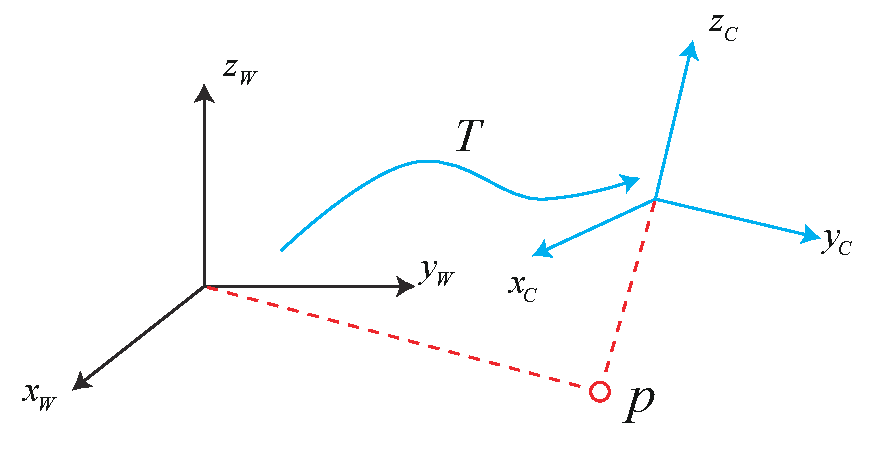
\includegraphics[width=0.7\textwidth]{rigidMotion/axisTransform.pdf}
    \caption {Coordinate transform. For the same vector $ \mathbf{p}$, its coordinates in the world $\mathbf{p}_W$ and the coordinates in the camera system $ \mathbf{p}_C$ are different. This transformation relationship is described by the transform matrix $ \mathbf{T} $.}
    \label{fig:axisTransform}
\end{figure}

Intuitively, the motion between two coordinate systems consists of a rotation plus a translation, which is called \textit{rigid body motion}. Obviously, the camera movement is rigid. During the rigid body motion, the length and angle of the vector will not change. Imagine you throw your phone into the air and \footnote {Please don't put it into practice because you may regret doing that.}, there may only be differences in spatial position and orientation. But the length and the angle of each face will not change. The phone will not be squashed like an eraser or be stretched during this motion. At this point, we say that the phone's motion is  \textit {Euclidean}.

The Euclidean transform consists of rotation and translation. Let's first consider the rotation. We have a unit-length orthogonal base $ ( \mathbf {e}_ 1, \mathbf {e}_ 2, \mathbf {e}_ 3 ) $. After a rotation it becomes $ ( \mathbf {e}_ 1 ', \mathbf {e}_ 2 ', \mathbf {e}_ 3 ') $. Then, for the same vector $ \mathbf {a} $ (the vector does not move with the rotation of the coordinate system), its coordinates in these two coordinate systems are $ [a_ 1, a_ 2, a_ 3 ] ^ \mathrm {T} $ and $[a'_ 1, a'_ 2, a'_ 3 ]^ \mathrm {T} $. Because the vector itself has not changed, according to the definition of coordinates, there are:

\begin{equation}
\left[ \mathbf{e}_1,\mathbf{e}_2,\mathbf{e}_3 \right]\left[ \begin{array}{l}
{a_1}\\
{a_2}\\
{a_3}
\end{array} \right] = \left[ \mathbf{e}_1', \mathbf{e}_2', \mathbf{e}_3' \right]\left[ \begin{array}{l}
a'_1\\
a'_2\\
a'_3
\end{array} \right].
\end{equation}

To describe the relationship between the two coordinates, we multiply the left and right sides of the above equation by $ \left [ \begin {array}{l}
\mathbf{e}_1^T\\
\mathbf{e}_2^T\\
\mathbf{e}_3^T
\end {array} \right ] $, then the matrix on the left becomes an identity matrix, so:

\begin{equation}
\left[ \begin{array}{l}
{a_1}\\
{a_2}\\
{a_3}
\end{array}\right]=\underbrace{\left[{\begin{array}{*{20}{c}}    
    {\mathbf{e}_1^T\mathbf{e}_1'} & {\mathbf{e}_1^T\mathbf{e}_2'} & {\mathbf{e}_1^T\mathbf{e}_3'}\\
    {\mathbf{e}_2^T\mathbf{e}_1'} & {\mathbf{e}_2^T\mathbf{e}_2'} & {\mathbf{e}_2^T\mathbf{e}_3'}\\
    {\mathbf{e}_3^T\mathbf{e}_1'} & {\mathbf{e}_3^T\mathbf{e}_2'} & {\mathbf{e}_3^T\mathbf{e}_3'}
    \end{array}} \right]}_{\text{rotation matrix}}\left[ \begin{array}{l}
a_1'\\
a_2'\\
a_3'
\end{array} \right] \buildrel \Delta \over = \mathbf{R} \mathbf{a}'.
\end{equation}
We take the intermediate matrix out and define it as a matrix $ \mathbf{R}$. This matrix consists of the inner product between the two sets of bases, describing the same vector's coordinate transformation relationship before and after the rotation. As long as the rotation is the same, this matrix is the same. It can be said that the matrix $ \mathbf{R} $ describes the rotation itself. So we call it the \textit{rotation matrix}. Meanwhile, the components of the matrix are the inner product of the two coordinate system bases. Since the base vector's length is 1, it is actually the cosine of the angle between the base vectors. So this matrix is also called \textit{direction cosine matrix}. We will just call it the rotation matrix in the following.

The rotation matrix has some special properties. In fact, it is an \textit{orthogonal} matrix with a determinant of 1 \footnote{Orthogonal matrix is a matrix whose inverse is its transpose. The orthogonality of the rotation matrix can be derived directly from the definition. } \footnote{The determinant is 1 is artificially defined. In fact, its determinant is $\pm 1 $, but the rotation with determinant $ - 1 $ is called \textit{improper rotation}, that is, one rotation plus one reflection in 3D space. }. Conversely, an orthogonal matrix with a determinant of 1 is also a rotation matrix. So, you can define a set of $n$ dimensional rotation matrices as follows:
\begin{equation}
\mathrm{SO}(n) = \{ \mathbf{R} \in \mathbb{R}^{n \times n} | \mathbf{R R}^T = \mathbf{I}, \mathrm{det} (\mathbf{R})=1 \}.
\end{equation}

$\mathrm{SO}(n) $ refers to the \textit {special orthogonal group}. We leave the contents of the ``group'' to the next lecture. This set consists of a rotation matrix of $ n $ dimensional space, in particular, $\mathrm {SO}(3)$ refers to the rotation of the three-dimensional space. In this way, we can talk directly about the rotation transformation between the two coordinate systems without having to start from the bases.

Since the rotation matrix is orthogonal, its inverse (i.e., transpose) describes an opposite rotation. According to the above definition, there are:
\begin{equation}
\mathbf{a} '= \mathbf{R}^{-1} \mathbf{a} = \mathbf{R}^{T} \mathbf{a}.
\end{equation}
Obviously the $ \mathbf{R}^T $ represents an opposite rotation.

In the Euclidean transformation, there is a translation in addition to the rotation. Consider the vector $ \mathbf{a} $ in the world coordinate system, after a rotation (depicted by $ \mathbf{R} $) and a translation of $ \mathbf{t} $, we get $ \mathbf{a}' $. Then we can put the rotation and translation together, and have:
\begin{equation}
\label{eq:RT}
\mathbf{a} '= \mathbf{R} \mathbf{a} + \mathbf{t},
\end{equation}
where $ \mathbf{t} $ is called a translation vector. Compared to the rotation, the translation part simply adds the translation vector to the coordinates after the rotation, which is very simple. By the above formula, we completely describe the coordinate transformation relationship using a rotation matrix $ \mathbf{R} $ and a translation vector $ \mathbf{t}$. In practice, we may define the coordinate system 1 and 2, then the vector $ \mathbf{a} $ under the two coordinates is $ \mathbf{a}_1, \mathbf{a}_2 $. The relationship between the two systems should be:
\begin{equation}
\mathbf{a}_1 = \mathbf{R}_{12} \mathbf{a}_2 + \mathbf{t}_{12}.
\end{equation}
Here $ \mathbf{R}_{12} $ means ``rotation of the vector from system 2 to system 1''. Since the vector is multiplied to the right of the rotation matrix, its subscript is \textit{read from right to left}. This is just a customary way of writing this book. Coordinate transformations are easy to confuse, especially if multiple coordinate systems exist. Similarly, if we want to express ``rotation matrix from 1 to 2'', we write it as $ \mathbf{R}_{21}$. The reader must be clear about the notation here, because different books may have different notations. Some notations about rotation will be denoted as the top left/subscript, and the text will be written on the right side.

About $\mathbf{t}_{12}$, readers may just take it as a translation vector without wondering about its physical meaning. In fact, it corresponds to a vector from the system 1's origin pointing to system 2's origin, and the coordinates are taken under system 1. So I suggest readers understand it as ``a vector from 1 to 2''. But the reverse $ \mathbf{t}_{21} $, which is a vector from 2's origin to 1's origin, whose \textit{coordinates are taken in system 2}, is not equal to $-\mathbf{t}_{12}$. It is also related to the rotation of the two systems. \footnote{Although they are indeed inverse relations from the vector level, the coordinates of the two vectors are not the opposite. Can you find out why it looks like this?} Therefore, when beginners ask the question ``What are my coordinates?'', we need to clearly explain this sentence's meaning. Here ``my coordinates'' normally refers to the vector from the world system $W$ pointing to the origin of the camera system $C$, and then take the coordinates in the world's base. Corresponding to the mathematical symbol, it should be the value of $ \mathbf{t}_{WC} $. For the same reason, it is not $ - \mathbf {t}_{CW}$, but actually $-\mathbf{R}_{CW}^T \mathbf{t}_{CW}$.

\subsection{Transform Matrix and Homogeneous Coordinates}
The formula~\eqref{eq:RT} fully expresses the rotation and translation of Euclidean space, but there is still a small problem: the transformation relationship here is not a linear relationship. Suppose we made two transformations: $ \mathbf {R}_ 1, \mathbf {t}_ 1 $ and $ \mathbf {R}_ 2, \mathbf {t}_ 2 $:
\[
\mathbf{b} = {\mathbf{R}_1} \mathbf{a} + {\mathbf{t}_1}, \quad \mathbf{c} = {\mathbf{R}_2} \mathbf{b} + {\mathbf{t}_2}.
\]
So, the transformation from $ \mathbf{a} $ to $ \mathbf{c} $ is:
\[
\mathbf{c} = {\mathbf{R}_2}\left( {{\mathbf{R}_1} \mathbf{a} + {\mathbf{t}_1}} \right) + {\mathbf{t}_2}.
\]
This form is not elegant after multiple transformations. Therefore, we introduce homogeneous coordinates and transformation matrices, rewriting the form~\eqref{eq:RT}:
\begin{equation}
\left[\begin{array}{l} 
\mathbf {a} ' \\
1
\end{array} \right] = 
\left[ {\begin{array}{*{20}{c}}
    \mathbf{R}&\mathbf{t}\\
    {{\mathbf{0}^T}}&1
    \end{array}} \right]
\left[ \begin{array}{l}
\mathbf {a} \\
1
\end{array} \right]  \buildrel \Delta \over = \mathbf{T} \left[ \begin{array}{l}
\mathbf {a} \\
1
\end{array} \right].
\end{equation}

This is a mathematical trick: we add $ 1 $ at the end of a 3D vector and turn it into a 4D vector called \textit{homogeneous coordinates}. For this four-dimensional vector, we can write the rotation and translation in one matrix, making the whole relationship a linear relationship. In this formula, the matrix $ \mathbf {T} $ is called \textit{transform matrix}.

We temporarily use $  \tilde { \mathbf {a} } $ to represent the homogeneous coordinates of $ \mathbf {a} $. Then, relying on homogeneous coordinates and transformation matrices, the superposition of the two transformations can have a good form:
\begin{equation}
\tilde{\mathbf{b}} = \mathbf{T}_1 \tilde{\mathbf{a}}, \  \tilde{\mathbf{c}} = \mathbf{T}_2 \tilde{\mathbf{b}} \quad \Rightarrow \tilde{\mathbf{c}} = \mathbf{T}_2 \mathbf{T_1} \tilde{\mathbf{a}}.
\end{equation}
But the symbols that distinguish between homogeneous and non-homogeneous coordinates are annoying, because here we only need to add 1 at the end of the vector or remove 1 to turn it into a normal vector \footnote {But the purpose of the homogeneous coordinates is not limited to this, we will come back to it in chapter~\ref{cpt:7}.}. So, without ambiguity, we will write it directly as $ \mathbf {b}= \mathbf {T} \mathbf {a} $, and by default we just assume a homogeneous coordinate conversion is made if needed \footnote { Note that if homogeneous coordinate transformation is not performed, the matrix multiplication here does not make sense. }.

The transformation matrix $\mathbf{T}$ has a special structure: the upper left corner is the rotation matrix, the right side is the translation vector, the lower-left corner is $ \mathbf{0} $ vector, and the lower right corner is 1. This set of transform matrix is also known as the \textit{special Euclidean group}:

\begin{equation}
\mathrm{SE}(3) = \left\{ \mathbf{T} = \left[ {\begin{array}{*{20}{c}}
    \mathbf{R} & \mathbf{t} \\
    {{\mathbf{0}^T}} & 1
    \end{array}} \right]
\in \mathbb{R}^{4 \times 4} | \mathbf{R} \in \mathrm{SO}(3), \mathbf{t} \in \mathbb{R}^3\right\} .
\end{equation}

Like $ \mathrm{SO}( 3 ) $, the inverse of the transform matrix represents an inverse transformation:

\begin{equation}
{ \mathbf{T}^{ - 1}} = \left[ {\begin{array}{*{20}{c}}
    {{\mathbf{R}^T}}&{ - {\mathbf{R}^T}\mathbf{t}}\\
    {{\mathbf{0}^T}}&1
    \end{array}} \right].
\end{equation}

Again, we use the notation of $ \mathbf{T}_{12} $ to represent a transformation from 2 to 1. Moreover, to keep the symbol concise, the symbols of the homogeneous coordinates and the ordinary coordinates are not deliberately distinguished in later sections in the case of no ambiguity. For example, when we write $ \mathbf {T} \mathbf{a} $, we use homogeneous coordinates (otherwise we can't calculate it). When we write $ \mathbf{Ra} $, we use non-homogeneous coordinates. If they are written in the same equation, it is assumed that the conversion from homogeneous coordinates to normal coordinates is already done - because the conversion between homogeneous and non-homogeneous coordinates is actually very easy. In C++ programs, we can simply do this with \textit{operator overloading} to ensure that the operations are correct.

Let's take a review now. First, we introduce the vector and its coordinate representation and introduce the operation between the vectors; then, the motion between the coordinate systems is described by the Euclidean transformation, which consists of translation and rotation. The rotation can be described by the rotation matrix $ \mathrm{SO}( 3 ) $, while the translation is directly described by an $ \mathbb{R}^ 3 $ vector. Finally, if the translation and rotation are placed in a matrix, the transformation matrix $ \mathrm{SE}( 3 ) $ is formed.

\section{Practice: Use \textit{Eigen}}
The practical part of this lecture has two sections. In the first part, we will explain how to use \textit{Eigen} to represent matrices and vectors and then extend to the calculation of rotation matrix and transformation matrix. The code for this section is in ``slambook2/ch3/useEigen''.

\textit{Eigen} \footnote{Official home page: \url{http://eigen.tuxfamily.org/index.php?title=Main_Page}. } is a C++ open-source linear algebra library. It provides fast linear algebra operations on matrices, as well as functions such as solving linear equations. Many upper-level software libraries also use \textit{Eigen} for matrix operations, including \textit{g2o}, Sophus, and others. Let's learn about \textit{Eigen}'s programming.

\textit{Eigen} may not have been installed on your PC. Please enter the following command to install it:

\begin{lstlisting}[language=sh,caption=Terminal input:]
sudo apt-get install libeigen3-dev
\end{lstlisting}

Most of the commonly used libraries in our book are available in the Ubuntu software center. With the apt command, we can easily install \textit{Eigen}. Looking back at the previous lesson, we know that a library consists of header files and library files. The \textit{Eigen} header file's default location should be  \textit{/usr/include/eigen3/}. If you are not sure, you can find it by entering the following command:

\begin{lstlisting}[language=sh,caption=Terminal input:]
sudo locate eigen3
\end{lstlisting}

\textit{Eigen} is a special library built with pure header files (this is the amazing part!). This means you can only locate its header files, not binary files like .so or .a. When you use it, you only need to import \textit{Eigen}'s header file. You don't need to link the library file (because it doesn't have any library files). Now let's write a piece of code below to actually practice the use of \textit{Eigen}:
\begin{lstlisting}[language=c++,caption=slambook2/ch3/useEigen/eigenMatrix.cpp]
#include <iostream>
using namespace std;

#include <ctime>
// Eigen core
#include <Eigen/Core>
// Algebraic operations of dense matrices (inverse, eigenvalues, etc.)
#include <Eigen/Dense>
using namespace Eigen;

#define MATRIX_SIZE 50

/****************************
* This program demonstrates the use of the basic Eigen type
****************************/

int main(int argc, char **argv) {
    // All vectors and matrices in Eigen are Eigen::Matrix, which is a template
    // class. Its first three parameters are: data type, row, column Declare a 2*3
    // float matrix
    Matrix<float, 2, 3> matrix_23;
    
    // At the same time, Eigen provides many built-in types via typedef, but the
    // bottom layer is still Eigen::Matrix. For example, Vector3d is essentially
    // Eigen::Matrix<double, 3, 1>, which is a three-dimensional vector.
    Vector3d v_3d;
    // This is the same
    Matrix<float, 3, 1> vd_3d;
    
    // Matrix3d is essentially Eigen::Matrix<double, 3, 3>
    Matrix3d matrix_33 = Matrix3d::Zero(); // initialized to zero
    // If you are not sure about the size of the matrix, you can use a matrix of
    // dynamic size
    Matrix<double, Dynamic, Dynamic> matrix_dynamic;
    // simpler
    MatrixXd matrix_x;
    // There are still many types of this kind. We don't list them one by one.
    
    // Here is the operation of the Eigen matrix
    // input data (initialization)
    matrix_23 << 1, 2, 3, 4, 5, 6;
    // output
    cout << "matrix 2x3 from 1 to 6: \n" << matrix_23 << endl;
    
    // Use () to access elements in the matrix
    cout << "print matrix 2x3: " << endl;
    for (int i = 0; i < 2; i++) {
        for (int j = 0; j < 3; j++)
        cout << matrix_23(i, j) << "\t";
        cout << endl;
    }
    
    // We can easily multiply a matrix with a vector (but actually still matrices and matrices)
    v_3d << 3, 2, 1;
    vd_3d << 4, 5, 6;
    
    // In Eigen you can't mix two different types of matrices, like this is
    // wrong Matrix<double, 2, 1> result_wrong_type = matrix_23 * v_3d; 
    // It should be explicitly converted
    Matrix<double, 2, 1> result = matrix_23.cast<double>() * v_3d;
    cout << "[1,2,3;4,5,6]*[3,2,1]=" << result.transpose() << endl;
    
    Matrix<float, 2, 1> result2 = matrix_23 * vd_3d;
    cout << "[1,2,3;4,5,6]*[4,5,6]: " << result2.transpose() << endl;
    
    // Also you can't misjudge the dimensions of the matrix
    // Try canceling the comments below to see what Eigen will report.
    // Eigen::Matrix<double, 2, 3> result_wrong_dimension =
    // matrix_23.cast<double>() * v_3d;
    
    // some matrix operations
    // The basic operations are not demonstrated, just use +-*/ operators.
    Matrix_33 = Matrix3d::Random(); // Random Number Matrix
    cout << "random matrix: \n" << matrix_33 << endl;
    cout << "transpose: \n" << matrix_33.transpose() << endl;
    cout << "sum: " << matrix_33.sum() << endl;
    cout << "trace: " << matrix_33.trace() << endl;
    cout << "times 10: \n" << 10 * matrix_33 << endl;
    cout << "inverse: \n" << matrix_33.inverse() << endl;
    cout << "det: " << matrix_33.determinant() << endl;
    
    // Eigenvalues
    // Real symmetric matrix can guarantee successful diagonalization
    SelfAdjointEigenSolver<Matrix3d> eigen_solver(matrix_33.transpose() *
	    matrix_33);
    cout << "Eigen values = \n" << eigen_solver.eigenvalues() << endl;
    cout << "Eigen vectors = \n" << eigen_solver.eigenvectors() << endl;
    
    // Solving equations
    // We solve the equation of matrix_NN * x = v_Nd
    // The size of N is defined in the previous macro, which is generated by a
    // random number Direct inversion is the most direct, but the amount of
    // inverse operations is large.
    
    Matrix<double, MATRIX_SIZE, MATRIX_SIZE> matrix_NN =
	    MatrixXd::Random(MATRIX_SIZE, MATRIX_SIZE);
    matrix_NN =
	    matrix_NN * matrix_NN.transpose(); // Guarantee semi-positive definite
    Matrix<double, MATRIX_SIZE, 1> v_Nd = MatrixXd::Random(MATRIX_SIZE, 1);
    
    Clock_t time_stt = clock(); // timing
    // Direct inversion
    Matrix<double, MATRIX_SIZE, 1> x = matrix_NN.inverse() * v_Nd;
    cout << "time of normal inverse is "
	    << 1000 * (clock() - time_stt) / (double)CLOCKS_PER_SEC << "ms" << endl;
    cout << "x = " << x.transpose() << endl;
    
    // Usually solved by matrix decomposition, such as QR decomposition, the speed
    // will be much faster
    time_stt = clock();
    x = matrix_NN.colPivHouseholderQr().solve(v_Nd);
    cout << "time of Qr decomposition is "
	    << 1000 * (clock() - time_stt) / (double)CLOCKS_PER_SEC << "ms" << endl;
    cout << "x = " << x.transpose() << endl;
    
    // For positive definite matrices, you can also use cholesky decomposition to
    // solve equations.
    time_stt = clock();
    x = matrix_NN.ldlt().solve(v_Nd);
    cout << "time of ldlt decomposition is "
	    << 1000 * (clock() - time_stt) / (double)CLOCKS_PER_SEC << "ms" << endl;
    cout << "x = " << x.transpose() << endl;
    
    return 0;
}
\end{lstlisting}

This example demonstrates the basic operations and operations of the \textit{Eigen} matrix. To compile it, you need to specify the header file directory of \textit{Eigen} in the \textit{CMakeLists.txt}:
\begin{lstlisting}[caption=slambook2/ch3/useEigen/CMakeLists.txt]
# Add header file
include_directories( "/usr/include/eigen3" )
\end{lstlisting}

Because the \textit{Eigen} library only has header files, we don't need to link the program to the library with the target\_link\_libraries statement. However, for most other libraries, you still need to use the link command. The approach here is not necessarily the best because others may have \textit{Eigen} installed in different locations, then you must manually modify the header file directory here. In the rest of the book, we will use the find\_ package command to search the library, but we keep it simple in this lecture. After compiling this program, run it, and you can see the output of each matrix.

\begin{lstlisting}[caption=Terminal output:]
% build/eigenMatrix
matrix 2x3 from 1 to 6: 
1 2 3
4 5 6
print matrix 2x3: 
1	2	3	
4	5	6	
[1,2,3;4,5,6]*[3,2,1]=10 28
[1,2,3;4,5,6]*[4,5,6]: 32 77
random matrix: 
0.680375   0.59688 -0.329554
-0.211234  0.823295  0.536459
0.566198 -0.604897 -0.444451
transpose: 
0.680375 -0.211234  0.566198
0.59688  0.823295 -0.604897
-0.329554  0.536459 -0.444451
sum: 1.61307
trace: 1.05922
times 10: 
6.80375   5.9688 -3.29554
-2.11234  8.23295  5.36459
5.66198 -6.04897 -4.44451
inverse: 
-0.198521   2.22739    2.8357
1.00605 -0.555135  -1.41603
-1.62213   3.59308   3.28973
it: 0.208598
\end{lstlisting}

Since the detailed comments are given in the code, we will not elaborate on each line of the statements. This book will only describe several important places (the latter part will also keep this style).

\begin{enumerate}
    \item Please enter the above code by yourself if you are a beginner in C++ (not including comments). At least compile and run the above program for once.
    
    \item KDevelop may not prompt C++ member functions, which is caused by its incompleteness. Please type the above contents just like what they are. Do not care if KDevelop prompts any errors. Clion's completion may be better. 
    
    \item Eigen's matrix is very similar to MATLAB, and almost all data is treated as a matrix. However, to achieve better efficiency, you need to specify the size and type of the \textit{Eigen} matrix. For matrices that we know the size at compile-time, they are processed faster than dynamically changing matrices. Therefore, data such as rotation matrices and transformation matrices can be determined at compile times by their size and data type.
    
    \item The matrix implementation inside  \textit{Eigen} is more complicated. I won't introduce it here. We hope you can use \textit{Eigen}'s matrix just like the built-in data types such as float and double.
    
    \item The \textit{Eigen} matrix does not support automatic type promotion, which is quite different from C++'s built-in data types. In a C++ program, we can add and multiply a float variable and double variable, and the compiler will automatically \textit{cast} the data type to the most appropriate one. In \textit{Eigen}, for performance reasons, you must explicitly convert the matrix type. And if you forget to do this, \textit{Eigen} will (not very friendly) prompt you with a very long ``YOU MIXED DIFFERENT NUMERIC TYPES ...'' compilation error. You can try to find out which part of the error message this message appears in. If the error message is too long, it is best to save it to a file and find it.
    
    \item At the same time, the calculation process also needs to ensure the correctness of the matrix dimension. Otherwise, there will be a ``YOU MIXED MATRICES OF DIFFERENT SIZES'' error. Please don't complain about this kind of error prompts. For C++ template meta-programming, it is very fortunate to have readable error information. Later, if you find some compilation error about \textit{Eigen}, you can directly look for the uppercase part and figure out the problem.
    
    \item Our example only covers the very basic matrix operations. You can learn more about \textit{Eigen} by reading the \textit{Eigen} official website tutorial: \\ { \url{http://eigen.tuxfamily.org/dox-devel/modules.html} }. Only the simplest part is demonstrated here. It is not equal to the fact that you can understand \textit{Eigen}.
\end{enumerate}

In the last piece of code, the efficiency of inversion and QR decomposition is compared. You can look at the time difference on your own machine. Is there a significant difference between the two methods?

\section{Rotation Vectors and the Euler Angles}
\subsection{Rotation Vectors}
Now let's return to the theoretical part. With a rotation matrix to describe the rotation, is it enough to use a $4 \times 4$ transformation matrix to represent a 6-degree-of-freedom 3D rigid body motion? Obviously, the matrix representation has at least the following disadvantages:
\begin{enumerate}
    \item  $\mathrm{SO}( 3 ) $ has a rotation matrix of 9 quantities, but a 3D rotation only has 3 degrees of freedom. Therefore the matrix expression is redundant. Similarly, the transformation matrix expresses a 6 degree-of-freedom transformation with 16 quantities. So, is there a more compact representation?
    \item The rotation matrix itself has constraints: it must be an orthogonal matrix with a determinant of 1. The same is true for the transformation matrix. These constraints make the solution more difficult when you want to estimate or optimize a rotation matrix/transform matrix.
\end{enumerate}

Therefore, we hope that there is a way to describe rotation and translation more compactly. For example, is it feasible to express the rotation with a three-dimensional vector and express transformation with a six-dimensional vector? Obviously, a rotation can be described by a rotation axis and a rotation angle. Thus, we can use a vector whose direction is parallel with the axis of rotation, and the length is equal to the angle of rotation, which is called the \textit{rotation vector} (or angle-axis/axis-angle). Only a three-dimensional vector is needed here to describe the rotation. Similarly, we may also use a rotation vector and a translation vector to express a transformation for a transformation matrix. The variable dimension at this time is exactly six dimensions.

Consider a rotation represented by $ \mathbf{R} $. If described by a rotation vector, assuming that the rotation axis is a unit-length vector $ \mathbf{n} $ and the angle is $ \theta $, then the vector $ \theta \mathbf{n} $ can also describe this rotation. So, we have to ask, what is the connection between the two expressions? In fact, it is not difficult to derive their conversion relationship. The conversion from the rotation vector to the rotation matrix is shown by the \textit{Rodrigues' formula}. Since the derivation process is a little complicated, it is not described here. Only the result of the conversion is given \footnote{For interested readers, please refer to \url{https://en.wikipedia.org/wiki/Rodrigues \% 27_rotation_formula}, in fact, the next chapter will give a brief proof from the Lie algebra view.}:

\begin{equation}
\label{eq:rogridues}
\mathbf{R} = \cos \theta \mathbf{I} + \left({ 1 - \cos \theta } \right) \mathbf{n} { \mathbf {n} ^T } + \sin \theta { \mathbf{n}^ \wedge }.
\end{equation}

The symbol $ ^ \wedge $ is a vector to skew-symmetric conversion, see the formula~\eqref{eq:cross}. Conversely, we can also calculate the conversion from a rotation matrix to a rotation vector. For the corner $ \theta $, taking the \textit{trace} of both sides\footnote {see \textit{trace} on both sides to find the sum of the diagonal elements of the matrix. }, we have:

\begin{equation}
\begin{aligned}
\mathrm{tr} \left( \mathbf{R} \right) &= \cos \theta \mathop{}\!\mathrm{tr}\left( \mathbf{I} \right) + \left( {1 - \cos \theta } \right) \mathop{}\!\mathrm{tr} \left( { \mathbf{n} {\mathbf{n}^T}} \right) + \sin \theta \mathop{}\!\mathrm{tr} ({\mathbf{n}^ \wedge })\\
&= 3\cos \theta  + (1 - \cos \theta )\\
&= 1 + 2\cos \theta .
\end{aligned} 
\end{equation}

Therefore:
\begin{equation}
\label{eq:R2theta}
\theta = \arccos \left( \frac{\mathrm{tr}(\mathbf{R}) - 1}{2}  \right) .
\end{equation}

Regarding the axis $ \mathbf{n} $, since the rotation axis does not change after the rotation, we have:
\begin{equation}
\mathbf{R} \mathbf{n} = \mathbf{n}.
\end{equation}

Therefore, the axis $ \mathbf{n} $ is the eigenvector corresponding to the matrix $ \mathbf{R}$'s eigenvalue 1. Solving this equation and normalizing it gives the axis of rotation. By the way, the two conversion formulas here will still appear in the next lecture, and you will find that they are exactly the correspondence between Lie group and Lie algebra on $ \mathrm{SO}(3) $ .

\subsection{Euler Angles}
Let's talk about the Euler angle.

Whether it is a rotation matrix or a rotation vector, although they can describe the rotation, it is hard to imagine what this rotation is like only with those numbers. When they change, we don't know which direction the object is turning. The Euler angle provides a very intuitive way to describe the rotation—it uses three primal axes to decompose a rotation into three rotations around different axes. Humans can easily understand the process of rotating around a single axis. However, due to the variety of decomposition methods, there are many alternative and confusing definitions of Euler angles. For example, we can first rotate around the $X$ axis, then the $Y$ axis, and finally around the $Z$ axis, and in this way, we get a rotation like $XYZ$ order. Similarly, you can define rotation orders such as $ZYZ$ and $ZYX$. You also need to distinguish whether it is rotated around the \textit{fixed axis} or around the \textit{axis after rotation}, which will also give a different definition.

This uncertainty in the axis orders brings many practical difficulties. Fortunately, in specific research areas, Euler angles usually have a uniform definition. You may have heard the words ``pitch angle'' and ``yaw angle'' of an aircraft. One of the most commonly used Euler angles is the yaw-pitch-roll angles. Since it is equivalent to the rotation of the $ZYX$ axis, we take the $ZYX$ Euler angle as an example. Suppose the front of a rigid body (toward our direction) is the $X$ axis, the right side is the $Y$ axis, and the top is the $Z$ axis, as shown by \autoref{fig:eulerAngles}. Then, the $ZYX$ angle is equivalent to decompose any rotation into the following three axes:

\begin{enumerate}
    \item Rotate around the $Z$ axis of the object to get the yaw angle $\theta_{\mathrm{yaw}}=y$;
    \item Rotate around the $Y$ axis of \textit{after rotation} to get the pitch angle $\theta_{\mathrm{pitch}}=p$;
    \item Rotate around the $X$ axis of \textit{after rotation} to get the roll angle $\theta_{\mathrm{roll}}=r$.
\end{enumerate}

\begin{figure}[!t]
    \centering
    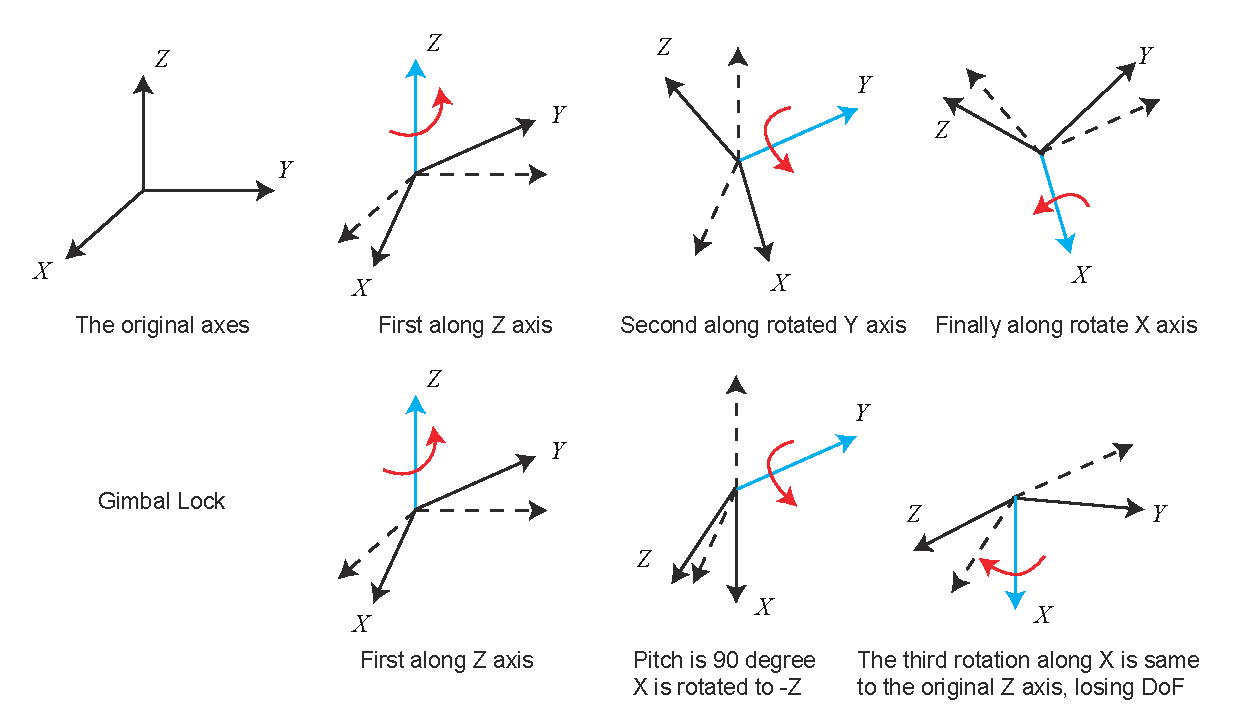
\includegraphics[width=1.0\textwidth]{rigidMotion/eulerAngles.pdf}
    \caption{Euler angles. The top is defined for the ZYX order (ypr order). The bottoms shows when pitch=$90^\circ$, the third rotation is using the same axis as the first one, causing the system to lose a degree of freedom. If you don't understand the gimbal lock, please take a look at the related videos and it will be more convenient to understand. }
    \label{fig:eulerAngles}
\end{figure}

In this way, we can use a three-dimensional vector such as $[y,p,r]^T$ to describe any rotation. This vector is very intuitive. We can imagine the rotation process from this vector. The other Euler angles are also decomposed into three axes to obtain a three-dimensional vector, but the axes and order may be different. The $ypr$ angle introduced here is a widely used one, and only a few Euler angles have such a famous name as $ypr$. Different Euler angles are referred to in the order of the axes of rotation. For example, the rotation order of the ypr angle is $ZYX$. Similarly, there are Euler angles like $XYZ, ZYZ$ - but they don't have a specific name. It is worth mentioning that most areas have their own coordinate directions and habits when using Euler angles, not necessarily the same as we said here.

A major drawback of Euler Angle is that it encounters the famous \textit{Gimbal lock} \footnote{See \url{https://en.wikipedia.org/wiki/Gimbal_lock}.}): in the $ypr$'s case, when the pitch angle is $\pm 90 ^\circ $, the first rotation and the third rotation will use the same axis, causing the system to lose a degree of freedom (from 3 rotations to 2 rotations). This is called the singularity problem and also exists in other forms of Euler angles. In theory, it can be proved that as long as you want to use three real numbers to express the three-dimensional rotation, you will inevitably encounter the singularity problem. \footnote{The rotation vector also has a singularity, which occurs when the angle $\theta$ exceeds $2\pi$. Obviously, rotating $2\pi$ is the same with no rotation.} Due to this fact, Euler angles are not suitable for interpolation or iterations, and are often only used in human-computer interaction. We rarely use Euler angles to express poses directly in the SLAM program, nor do we use Euler angles to describe rotation in filtering or optimization (because it has singularity). However, if you want to verify that your algorithm is correct or not, converting to Euler angles can help you quickly determine if the results are correct or not. In some cases where the main body is mainly 2D motion (such as sweepers, self-driving vehicles), we can also decompose the rotation into three Euler angles and then take one of them (such as the yaw angle) as the orientation output.

\section{Quaternions}
The rotation matrix describes 3 degrees of freedom with 9 quantities, of course, with redundancy; the Euler angles and the rotation vectors are compact but suffer from the singularity. In fact, we \textit{cannot} find a three-dimensional vector description without singularity~\cite{Stuelpnagel1964}. This is somewhat similar to using two coordinates to represent the Earth's surface (such as longitude and latitude), which also has the singularity (longitude is meaningless when the latitude is $ \pm  90 ^ \circ $ ).

Recall the complex number that we have studied before. We use the complex set $ \mathbb {C} $ to represent the vector on the 2D complex plane, and the complex multiplication with a unit complex number can represent the rotation on the 2D plane: for example, multiplying the complex $i$ is equivalent to rotating a complex vector counterclockwise by $ 90 ^ \circ $. Similarly, when expressing a three-dimensional space rotation, there is also an algebra similar to a complex number: the \textit{quaternions}. Quaternions are extended complex numbers found by Hamilton. It is both compact and not singular. If we must find some shortcomings, the quaternion is not intuitive enough, and its operation is a bit more complicated.

Comparing quaternions to complex numbers can help you understand quaternions faster. For example, when we want to rotate the vector of a complex plane by $\theta$, we can multiply this complex vector by $\mathrm{e}^{i \theta}$, which is represented by polar coordinates. It can also be written in the usual form like the famous Euler equation:
\begin{equation}
\mathrm{e}^{i\theta} = \cos \theta + i \sin \theta.
\end{equation}
This is a unit-length complex number. Therefore, in two dimensions, the rotation can be described by a unit complex number. Similarly, we will see that 3D rotation can be described by a unit quaternion.

A quaternion $ \mathbf{q} $ has a real part and three imaginary parts. We write the real part in the front (and there are also some books where the real part is in the last), like this:
\begin{equation}
\mathbf{q} = q_0 + q_1 i + q_2 j + q_3 k,
\end{equation}
where $ i,j,k $ are three imaginary parts of the quaternion. These three imaginary parts satisfy the following relationship:
\begin{equation}
\label{eq:quaternionVirtual}
\left\{ \begin{array}{l}
{i^2} = {j^2} = {k^2} =  - 1\\
ij = k, ji = - k \\
jk = i,kj =  - i\\
ki = j, ik = - j
\end{array} \right. .
\end{equation}
If we look at $ i, j, k $ as three axes, they look the same as complex numbers when multiplying with themselves. And look the same as the outer product when multiplying with the others. 

We can also use a scalar and a vector to express quaternions:
\[
\mathbf{q} = \left[ s, \mathbf{v} \right]^T, \quad s=q_0 \in \mathbb{R},\quad \mathbf{v} = [q_1, q_2, q_3]^T \in \mathbb{R}^3,
\]
Here, $ s $ is the real part of the quaternion, and $ \mathbf {v} $ is its imaginary part. If the imaginary part of a quaternion is $ \mathbf {0} $, it is called \textit{real quaternion}. Conversely, if its real part is $ 0 $, it is called \textit{imaginary quaternion}.

We can use a unit quaternion to represent any rotation in 3D space, but this expression is subtly different from the complex numbers. In the complex, multiplying by $ i $ means rotating $ 90 ^ \circ $. Does this mean that in the quaternion, multiplied by $ i $ is rotating around the $ i $ axis by $ 90 ^ \circ $ ? So, does $ ij = k $ means, first rotating around the $ i $ by $ 90 ^ \circ $, then around $j$ by $ 90 ^ \circ $, is equivalent to rotating around $ k$ by $ 90 ^ \circ $ ? Readers can use a cell phone to simulate that, then you will find that this is not the right case. The correct situation should be that multiplying $ i $ corresponds to rotating $ 180 ^ \circ $, in order to guarantee the nature of $ ij=k $. And $ i^ 2 =- 1 $ means that after rotating $ 360 ^ \circ $ around the $ i $ axis, we get an opposite thing. This object has to be rotated by 720 $^\circ$ to be equal to its original appearance.

This seems a bit mysterious. The complete explanation needs too many extra things. Let's calm down and come back to the quaternions. At least, we know that a unit quaternion can express the rotation of a three-dimensional space. So what are the properties of the quaternions? And how can they operate with each other?

\subsection{Quaternion Operations}
Quaternions are very similar to complex numbers, and a series of quaternion operations can be performed. We can easily plus, minus, multiplies to quaternions just like doing with two complex numbers. Assume there are two quaternions $ \mathbf{q}_a, \mathbf{q}_b $, whose vectors are represented as $ [s_a, \mathbf {v}_a]^ \mathrm {T}, [s_b, \mathbf{v}_b]^ \mathrm {T} $, or the original quaternion is expressed as:
\[
\mathbf{q} _a = s_a + x_ai + y_aj + z_ak, \quad  \mathbf {q} _b = s_b + x_bi + y_bj + z_bk.
\]
Then, their operations can be expressed as follows.

\begin{enumerate}
    \item { \textbf{Addition and subtraction}.} The addition and subtraction of the quaternion $ \mathbf {q}_a, \mathbf {q}_b $ is:
    \begin{equation} 	
    \mathbf{q}_a \pm \mathbf{q}_b = \left[ s_a \pm s_b, \mathbf{v}_a \pm \mathbf{v}_b \right]^T.
    \end{equation}
    \item { \textbf {Multiplication}}. Quaternion multiplication is the multiplication of each item of $ \mathbf {q}_a $ with each item of $ \mathbf {q}_b $. The imaginary part is done according to  formula~\eqref {eq:quaternionVirtual}:
    \begin{equation}
    \begin{aligned}
    \mathbf{q}_a \mathbf{q}_b &= {s_a}{s_b} - {x_a}{x_b} - {y_a}{y_b} - {z_a}{z_b}\\
    &+ \left( {{s_a}{x_b} + {x_a}{s_b} + {y_a}{z_b} - {z_a}{y_b}} \right)i\\
    &+ \left( {{s_a}{y_b} - {x_a}{z_b} + {y_a}{s_b} + {z_a}{x_b}} \right)j\\
    &+ \left( {{s_a}{z_b} + {x_a}{y_b} - {y_a}{x_b} + {z_a}{s_b}} \right)k.
    \end{aligned}
    \end{equation}
    
    The scalar form is a little complicated, but the vector form is more concise:
    \begin{equation}
    \mathbf{q}_a \mathbf{q}_b = \left[ s_a s_b - \mathbf{v}_a^T \mathbf{v}_b, s_a\mathbf{v}_b + s_b\mathbf{v}_a + \mathbf{v}_a \times \mathbf{v}_b \right]^T.
    \end{equation}
    
    Under this multiplication definition, the product of two real quaternions is still real, which is also consistent with the real number multiplication. However, note that due to the existence of the last outer product, quaternion multiplication is usually not commutative unless $ \mathbf {v}_a $ and $ \mathbf {v}_b $ at $ \mathbb {R}^ 3 $ are parallel, which means the outer product term is zero.
    
    \item { \textbf {Length}. } The length of a quaternion is defined as:
    \begin{equation}
    \| \mathbf{q}_a \| = \sqrt{ s_a^2 + x_a^2 + y_a^2 + z_a^2 }.
    \end{equation}
    It can be verified that the length of the product is the product of the lengths. This makes the unit quaternion keep unit-length when multiplied by another unit quaternion:
    \begin{equation}
    \| \mathbf{q}_a \mathbf{q}_b \| = \|\mathbf{q}_a \| \| \mathbf{q}_b \|.
    \end{equation}
    
    \item { \textbf {Conjugate}}. The conjugate of a quaternion is to take the imaginary part as the opposite:
    \begin{equation}
    \mathbf{q}_a ^ * = s_a - x_ai - y_aj - z_ak = [s_a, - \mathbf{v}_a] ^T.
    \end{equation}
    We get a real quaternion if the quaternion is multiplied by its conjugate. The real part is the square of its length:
    \begin{equation}
    \mathbf{q}^* \mathbf{q} = \mathbf{q} \mathbf{q}^* = [s^2+\mathbf{v}^T \mathbf{v}, \mathbf{0} ]^T.
    \end{equation}
    
    \item { \textbf{Inverse}}. The inverse of a quaternion is:
    \begin{equation}
    \label{eq:quaternionInverse}
    \mathbf{q} ^ { - 1 } = \mathbf{q} ^ * / \| \mathbf{q} \| ^ 2.
    \end{equation}
    According to this definition, the product of the quaternion and its inverse is the real quaternion $ \mathbf {1} $ :
    \begin{equation}
    \mathbf{q} \mathbf{q}^{-1} = \mathbf{q}^{-1} \mathbf{q} = \mathbf{1}.
    \end{equation}
    
    If $ \mathbf{q} $ is a unit quaternion, its inverse and conjugate are the same. So the inverse of the product has properties similar to matrices:
    \begin{equation}
    \left( \mathbf{q}_a \mathbf{q}_b \right)^{-1} = \mathbf{q}_b^{-1} \mathbf{q}_a^{-1}.
    \end{equation}
    
    \item { \textbf {Scalar Multiplication}.} Similar to vectors, quaternions can be multiplied by numbers:
    \begin{equation}
    k \mathbf{q} = \left[ ks, k\mathbf{v} \right]^T.
    \end{equation}
\end{enumerate}

\subsection{Use Quaternion to Represent a Rotation}

We can use a quaternion to express the rotation of a point. Suppose a spatial 3D point $ \mathbf{p} = [x,y,z]^T \in  \mathbb {R}^3$, and a rotation is specified by a unit quaternion $ \mathbf{q}$. The 3D point $\mathbf{p}$ is rotated to become $\mathbf{p}'$. If we use matrix, then there is $ \mathbf{p}'= \mathbf{R} \mathbf{p} $. And if we use quaternion to describe rotation, how do we operate a 3D vector with a quaternion?

First, we extend the 3D point to an imaginary quaternion:
\[
\mathbf{p} = [0, x, y, z]^T = [0, \mathbf{v}]^T. 
\]
We just put the three coordinates into the imaginary part and leave the real part to be zero. Then, the rotated point $ \mathbf {p}' $ can be expressed as such a product:

\begin{equation}\label{eq:rotate-with-quaternion}
\mathbf{p}' = \mathbf{q} \mathbf{p} \mathbf{q}^{-1}.
\end{equation}

The multiplication here is the quaternion multiplication, and the result is also a quaternion. Finally, we take the imaginary part of $ \mathbf{p}' $ and get the coordinates of the point after the rotation. It can be easily verified (we leave as an exercise here) that the real part of the calculation is 0, so it is a pure imaginary quaternion.

\subsection{Conversion of Quaternions to Other Rotation Representations}

An arbitrary unit quaternion describes a rotation, which can also be described by a rotation matrix or a rotation vector. Now let's examine the conversion relationship between quaternions and rotation vectors/matrices. Before that, we have to say that quaternion multiplication can also be written as a matrix multiplication. Let $\mathbf{q}=[s,\mathbf{v}]^T$, then define the following symbols $^{+}$ and $^{\oplus}$ as~\cite{Barfoot2011}:
\begin{equation}
	\mathbf{q}^{+}=\left[\begin{array}{cc}
		s&-\mathbf{v}^T \\
		\mathbf{v}&s\mathbf{I}+\mathbf{v}^{\wedge}
	\end{array}\right],\quad
	\mathbf{q}^{\oplus}=
	\left[\begin{array}{cc}
		s & -\mathbf{v}^T \\
		\mathbf{v} & s\mathbf{I}-\mathbf{v}^{\wedge}
	\end{array}\right],
\end{equation}
These two symbols map the quaternion to a 4$\times$4 matrix. Then the quaternion multiplication can be written in the form of a matrix:
\begin{equation}
	\mathbf{q}_1^ + {\mathbf{q}_2} = \left[ {\begin{array}{*{20}{c}}
			s_1&-\mathbf{v}_1^T\\
			\mathbf{v}_1 & s_1 \mathbf{I} + \mathbf{v}_1^\wedge
	\end{array}} \right]\left[ {\begin{array}{*{20}{c}}
			{{s _2}} \\
			{{\mathbf{v} _2}}
	\end{array}} \right] = \left[ {\begin{array}{*{20}{c}}
			{ - \mathbf{v} _1^T{\mathbf{v} _2} + {s _1}{s _2}} \\
			{{s _1}{\mathbf{v} _2} + {s _2}{\mathbf{v} _1} + \mathbf{v} _1^ \wedge {\mathbf{v} _2}}
	\end{array}} \right] = \mathbf{q}_1 \mathbf{q}_2
\end{equation}
Note that the left side is matrix multiplication and the right side is quaternion multiplication. Similar for $^\oplus$, we get:
\begin{equation}
	\mathbf{q}_1 \mathbf{q}_2 = \mathbf{q}_1^{+} \mathbf{q}_2 = \mathbf{q}_2^{\oplus} \mathbf{q}_1.
\end{equation}

Then, consider the problem of using a quaternion to rotate a spatial point. According to the previous section, we have:
\begin{equation}
	\begin{split}
		\mathbf{p}' &= \mathbf{q} \mathbf{p} \mathbf{q}^{-1} = \mathbf{q}^+ \mathbf{p}^+ \mathbf{q}^{ -1} \\
		&= \mathbf{q}^+ \mathbf{q}^{{-1}^{\oplus}} \mathbf{p}.
	\end{split}
\end{equation}
Substituting the matrix corresponding to two symbols, we get:
\begin{equation}\label{eq:quaternion-to-rotation-matrix-derive}
	{\mathbf{q}^ + }{\left( {{\mathbf{q}^{ - 1}}} \right)^ \oplus } = \left[ \begin{array}{*{20}{c }}
		s&-\mathbf{v}^T\\
		\mathbf{v}&s\mathbf{I}+\mathbf{v}^\wedge
	\end{array} \right]\left[\begin{array}{*{20}{c}}
		s&{\mathbf{v} ^T}\\
		{ - \mathbf{v} }&{s\mathbf{I} + \mathbf{v} ^ \wedge }
	\end{array} \right] = \left[ \begin{array}{*{20}{c}}
		1&\mathbf{0} \\
		\mathbf{0}^T&\mathbf{v}\mathbf{v}^T + {s^2} \mathbf{I} + 2s\mathbf{v} ^ \wedge + {(\mathbf{v} ^ \wedge)}^2
	\end{array} \right].
\end{equation}
Since $\mathbf{p}'$ and $\mathbf{p}$ are both imaginary quaternions, so in fact that the bottom right corner of the matrix gives the transformation formula \textit{from quaternion to rotation matrix} :
\begin{equation}
	\mathbf{R} = \mathbf{v} \mathbf{v}^T + {s^2} \mathbf{I} + 2s\mathbf{v} ^ \wedge + {(\mathbf{v } ^ \wedge)}^2.
\end{equation}
In order to obtain the conversion formula of the quaternion to the rotation vector, we take the trace on both sides of the above formula:
\begin{equation}
	\begin{aligned}
		\mathrm{tr}(\mathbf{R}) &= \mathrm{tr}(\mathbf{v}\mathbf{v}^T) + 3s^2 + 2s \cdot 0 + \mathrm{tr }((\mathbf{v}^\wedge)^2) \\
		&= v_1^2+v_2^2+v_3^2 + 3s^2 - 2(v_1^2+v_2^2+v_3^2) \\
		&= (1-s^2) + 3s^2 -2(1-s^2)\\
		&= 4s^2 -1.
	\end{aligned}
\end{equation}
Also obtained by the formula~\eqref{eq:R2theta}:
\begin{equation}
	\begin{aligned}
		\theta &= \arccos\left(\frac{\mathrm{tr}(\mathbf{R})-1}{2}\right) \\
		&=\arccos(2s^2-1),
	\end{aligned}
\end{equation}
which means:
\begin{equation}
	\cos \theta =2s^2-1=2 \cos^2 \frac{\theta}{2} -1,
\end{equation}
and so we have:
\begin{equation}
	\theta = 2 \arccos s.
\end{equation}
For the rotation axis, if we replace $\mathbf{p}$ with the imaginary part of $\mathbf{q}$ in the formula~\eqref{eq:quaternion-to-rotation-matrix-derive}, it is easy to know the imaginary part of  $\mathbf{q}$ is not moving when it is rotated, that is, it constitutes exactly the rotation axis. So we get the rotation axis just by normalizing $\mathbf{q}$'s imaginary part. In summary, the conversion formula from quaternion to rotation vector can be written as follows:
\begin{equation}
	\label{eq:rotationVector2Quaternion}
	\begin{cases}
		\theta = 2\arccos {q_0}\\
		{\left[ {{n_x},{n_y},{n_z}} \right]^T} = {{{\left[ {{q_1},{q_2},{q_3}} \right] }^T}}/{\sin \frac{\theta }{2}}
	\end{cases} .
\end{equation}

And for converting from other representations to quaternions, we only need to reversely follow the above steps. In actual programming, the library usually prepares for the conversion between various forms for us. Whether it's a quaternion, a rotation matrix, or an angle-axis, it can always be used to describe the same rotation. We should choose the most convenient form in practice without having to stick to a particular form. In the subsequent practices and exercises, we will demonstrate the transition between various expressions to deepen the reader's impression.

\section{Affine and Projective Transformation}
In addition to the Euclidean transformation, there are several other transformations in the 3D space, where the Euclidean is the simplest. Some of them are related to camera geometry. We will introduce them in the following chapters, so here we only list their basic properties. The Euclidean transformation keeps the vector's length and angle, which is equivalent to moving or rotating a rigid body without changing its appearance. The other transformations will change their shape, and they all have similar matrix representations.

\begin{enumerate}
	\item {\textbf{Similarity transformation}}.
	
	The similarity transformation has one more degree of freedom than the Euclidean transformation, which allows the object to be uniformly scaled, and its matrix is expressed as:
	\begin{equation}
	\mathbf{T}_S = \left[ {\begin{array}{*{20}{c}}
		{s \mathbf{R}}& \mathbf{t}\\
		{{ \mathbf{0}^T}}&1
		\end{array}} \right].
	\end{equation}
	
	Note that the rotation part has an extra scaling factor $s$, which means that we can evenly scale the three coordinates of $x,\ y,\ and\ z$ of a vector after it is rotated. Due to the scaling, a similarity transformation no longer keeps the volume of the transformed boy unchanged. You can imagine a cube with a side length of 1 transforming into a side with a length of 10 (but still being a cube). The set of three-dimensional similarity transform is also called \textit{similarity transform group}, which is denoted as $\mathrm{Sim}(3)$.
	
	\item {\textbf{Affine transformation}}.
	
	The matrix form of the affine transformation is as follows:
	\begin{equation}
	\mathbf{T}_A = \left[ {\begin{array}{*{20}{c}}
		\mathbf{A} & \mathbf{t}\\
		{{\mathbf{0}^T}} & 1
		\end{array}} \right].
	\end{equation}
	

	Unlike the Euclidean transformation, the affine transformation requires only $\mathbf{A}$ to be an invertible matrix, not necessarily an orthogonal matrix. An affine transformation is also called an orthogonal projection. After the affine transformation, the cube is no longer square, but the faces are still parallelograms.	
	
	\item{ \textbf{Perspective transformation}. }
	
	Perspective transformation is the most general transformation. Its matrix form is:
	
	\begin{equation}
	{\mathbf{T}_P} = \left[ {\begin{array}{*{20}{c}}
		\mathbf{A} & \mathbf{t}\\
		{{\mathbf{a}^T}} & v
		\end{array}} \right].
	\end{equation}
	
	Its upper left corner is the invertible matrix $\mathbf{A}$. The upper right corner is the translation $\mathbf{t}$, and the lower-left corner is the scale $\mathbf{a}^T$. Since the homogeneous coordinates are used, when $v \neq 0$, we can divide the entire matrix by $v$ to get a matrix with a bottom right corner of 1; otherwise, we get a matrix with a lower right corner of $0$. Therefore, the 2D perspective transformation has a total of 8 degrees of freedom, and 3D has a total of 15 degrees of freedom. Perspective transformation is the most general transformation that has been said so far. The transformation from the real world to a camera photo can be seen as a perspective transformation. The reader can imagine what a square tile would look like in a photo: first, it is no longer square. Second, since the close part is larger than the far-away part, it is not even a parallelogram but an irregular quadrilateral. 
\end{enumerate}

\autoref{table:common-transform} summarizes the properties of several transformations currently covered. Note that in the ``invariance'', there is an inclusion relationship from top to bottom. For example, in addition to maintaining volume, the Euclidean transformation also keeps the parallelism, intersection, and others.

\begin{table}[!htp]
	\centering
	\caption{comparison of common transformation properties}
	\label{table:common-transform}
	\small
	\begin{tabular}{c|c|c|c}
		\toprule
		Transform Name & Matrix Form & Degrees of Freedom & Invariance \\ \midrule
		Euclidean \rule{0pt}{20 pt} & $\left[ {\begin{array}{*{20}{c}}
			\mathbf{R} & \mathbf{t}\\
			{{\mathbf{0}^T}}&1
			\end{array}} \right]$ & 6 & Length, angle, volume \\
		Similarity \rule{0pt}{20 pt}& $ \left[ {\begin{array}{*{20}{c}}
			{s \mathbf{R}}& \mathbf{t}\\
			{{ \mathbf{0}^T}}&1
			\end{array}} \right]$ & 7 & volume ratio \\
		Affine \rule{0pt}{20 pt}& $ \left[ {\begin{array}{*{20}{c}}
			\mathbf{A} & \mathbf{t}\\
			{{\mathbf{0}^T}} & 1
			\end{array}} \right]$ & 12 & Parallelism, volume ratio \\
		Perspective \rule{0pt}{20 pt} & $ \left[ {\begin{array}{*{20}{c}}
			\mathbf{A} & \mathbf{t}\\
			{{\mathbf{a}^T}} & v
			\end{array}} \right]$ & 15 & Plane intersection and tangency \rule{0pt}{20 pt}\\
		\bottomrule
	\end{tabular}
\end{table}

We will introduce later that the transformation from the real world to the camera photo is a perspective transformation. If the focal length of the camera is infinity, then this transformation is affine. However, before we go into the camera model's details, let's do some experiments to have a rough impression of these transformations.

\section{Practice: \textit{Eigen} Geometry Module}
\subsection{Data Structure of the \textit{Eigen} Geometry Module}
Now, let's actually practice the various rotation expressions mentioned earlier. We will use quaternions, Euler angles, and rotation matrices in \textit{Eigen} to demonstrate how they are transformed. We will also provide a visualization program to help the reader understand the relationship between these transformations.

\begin{lstlisting}[language=c++,caption=slambook2/ch3/useGeometry/useGeometry.cpp]
#include <iostream>
#include <cmath>
using namespace std;

#include <Eigen/Core>
#include <Eigen/Geometry>

using namespace Eigen;
// This program demonstrates how to use the Eigen geometry module

int main(int argc, char **argv) {
	// The Eigen/Geometry module provides a variety of rotation and translation representations
	// 3D rotation matrix directly using Matrix3d or Matrix3f
	Matrix3d rotation_matrix = Matrix3d::Identity();
	// The rotation vector uses AngleAxis, the underlying layer is not directly Matrix, but the operation can be treated as a matrix (because the operator is overloaded)
	AngleAxisd rotation_vector(M_PI / 4, Vector3d(0, 0, 1)); // Rotate 45 degrees along the Z axis
	cout.precision(3);
	cout << "rotation matrix = \n " << rotation_vector.matrix() << endl; // convert to matrix with matrix()
	// can also be assigned directly
	rotation_matrix = rotation_vector.toRotationMatrix();
	// coordinate transformation with AngleAxis
	Vector3d v(1, 0, 0);
	Vector3d v_rotated = rotation_vector * v;
	cout << "(1,0,0) after rotation (by angle axis) = " << v_rotated.transpose() << endl;
	// Or use a rotation matrix
	v_rotated = rotation_matrix * v;
	cout << "(1,0,0) after rotation (by matrix) = " << v_rotated.transpose() << endl;
	
	// Euler angle: You can convert the rotation matrix directly into Euler angles
	Vector3d euler_angles = rotation_matrix.eulerAngles(2, 1, 0); // ZYX order, ie roll pitch yaw order
	cout << "yaw pitch roll = " << euler_angles.transpose() << endl;
	
	// Euclidean transformation matrix using Eigen::Isometry
	Isometry3d T = Isometry3d::Identity(); // Although called 3d, it is essentially a 4*4 matrix
	T.rotate(rotation_vector); // Rotate according to rotation_vector
	T.pretranslate(Vector3d(1, 3, 4)); // Set the translation vector to (1,3,4)
	cout << "Transform matrix = \n" << T.matrix() << endl;
	
	// Use the transformation matrix for coordinate transformation
	Vector3d v_transformed = T * v; // Equivalent to R*v+t
	cout << "v tranformed = " << v_transformed.transpose() << endl;
	
	// For affine and projective transformations, use Eigen::Affine3d and Eigen::Projective3d.
	
	// Quaternion
	// You can assign AngleAxis directly to quaternions, and vice versa
	Quaterniond q = Quaterniond(rotation_vector);
	cout << "quaternion from rotation vector = " << q.coeffs().transpose() << endl; 
	// Note that the order of coeffs is (x, y, z, w), w is the real part, the first three are the imaginary part
	// can also assign a rotation matrix to it
	q = Quaterniond(rotation_matrix);
	cout << "quaternion from rotation matrix = " << q.coeffs().transpose() << endl;
	// Rotate a vector with a quaternion and use overloaded multiplication
	V_rotated = q * v; // Note that the math is qvq^{-1}
	cout << "(1,0,0) after rotation = " << v_rotated.transpose() << endl;
	// expressed by regular vector multiplication, it should be calculated as follows
	cout << "should be equal to " << (q * Quaterniond(0, 1, 0, 0) * q.inverse()).coeffs().transpose() << endl;
	
	return 0;
}
\end{lstlisting}

The various forms of expression in \textit{Eigen} are summarized below. Note that each type has both single and double precision types and, as before, cannot be automatically converted by the compiler. Taking the double-precision as an example, you can simply change the last ``d'' to ``f'' to use a single-precision data structure.
\begin{itemize}
	\item Rotation matrix ( $ 3  \times  3 $ ): Eigen::Matrix3d.
	\item Rotation vector ( $ 3  \times  1 $ ): Eigen::AngleAxisd.
	\item Euler angle ( $ 3  \times  1 $ ): Eigen::Vector3d.
	\item Quaternion ( $ 4  \times  1 $ ): Eigen::Quaterniond.
	\item Euclidean transformation matrix ( $ 4  \times  4 $ ): Eigen::Isometry3d.
	\item Affine transform ( $ 4  \times  4 $ ): Eigen::Affine3d.
	\item Perspective transformation ( $ 4  \times  4 $ ): Eigen::Projective3d.
\end{itemize}

This program can be compiled by referring to the corresponding ``CMakeLists.txt'' in the code. This program demonstrates how to use the rotation matrix, rotation vectors (AngleAxis), Euler angles, and quaternions in \textit{Eigen}. We use these rotations to rotate a vector $ \mathbf {v} $ and find that the result is the same. At the same time, it also demonstrates how to convert these expressions in the program. Readers who want to learn more about \textit{Eigen}'s geometry modules can refer to \url {http://eigen.tuxfamily.org/dox/group__TutorialGeometry.html}.

Note that the code has some subtle differences from the mathematical representation. For example, by operator overloading in C++, quaternions and three-dimensional vectors can directly be multiplied, but mathematically, the vector needs to be converted into an imaginary quaternion, as we talked about in the last section, and then quaternion multiplication is used for calculation. The same applies to the transformation matrix multiplying with a three-dimensional vector. In general, the usage in the program is more flexible than the mathematical formula.

\subsection{Coordinate Transformation Example}

Let's take a small example to demonstrate the coordinate transformation.

\noindent  \textit{Example 1}. \quad  The robot No.1 and the robot No.2 are located in the world coordinate system. We use the world coordinate system as $W$, robot coordinate system as $R_1 $ and $R_2$. The pose of the robot 1 is $ \mathbf {q}_ 1 = [ 0.35, 0.2, 0.3, 0.1 ]^T, \mathbf{t}_ 1 = [ 0.3, 0.1, 0.1 ]^T $. The pose of the robot 2 is $ \mathbf{q}_2 = [ - 0.5, 0.4, - 0.1, 0.2 ]^T, \mathbf{t}_ 2 = [- 0.1, 0.5, 0.3 ]^T $. Here $ \mathbf {q} $ and $ \mathbf{t} $ express $ \mathbf{T}_{R_k, W}, k= 1, 2 $, which is the world to the robot transform matrix. Now, assume that robot 1 sees a point in its own coordinate system with coordinates of $ \mathbf{p}_{R_1} = [ 0.5, 0, 0.2 ]^T $. We want to find the coordinates of the vector in the robot 2's coordinate system.

This is a very simple but representative example. In real scenarios you often need to convert coordinates between different parts of the same robot or between different robots. Below we write a program to demonstrate this calculation.

\begin{lstlisting}[language=c++,caption=slambook2/ch3/examples/coordinateTransform.cpp]
#include<iostream>
#include<vector>
#include<algorithm>
#include<Eigen/Core>
#include<Eigen/Geometry>

using namespace std;
using namespace Eigen;

int main(int argc, char** argv) {
	Quaterniond q1(0.35, 0.2, 0.3, 0.1), q2(-0.5, 0.4, -0.1, 0.2);
	q1.normalize();
	q2.normalize();
	Vector3d t1(0.3, 0.1, 0.1), t2(-0.1, 0.5, 0.3);
	Vector3d p1(0.5, 0, 0.2);
	
	Isometry3d T1w(q1), T2w(q2);
	T1w.pretranslate (t1);
	T2w.pretranslate (t2);
	
	Vector3d p2 = T2w * T1w.inverse() * p1;
	cout << endl << p2.transpose() << endl;
	return 0;
}
\end{lstlisting}

The answer to the program is $ [- 0.0309731, 0.73499, 0.296108 ]^T$, and the calculation process is very simple, just by calculating $$ \mathbf{p}_{R_2} = \mathbf{T}_{ R_2, W} \mathbf{T}_{W, R_1} \mathbf{p}_{R_1}. $$ Note that the quaternion needs to be normalized before use.

\section{Visualization Demo}
\subsection{Plotting Trajectory}
If you are new to rotation and translation concepts, you may find that their form looks a little complicated. There are so many representation methods, and we need to convert to a preferred one if necessary. Fortunately, although the rotation and transformation matrix values may not be intuitive enough, we can easily draw them in a 3D window.

In this section, we demonstrate two visual examples. First, let's say that we recorded the trajectory of a robot somehow, and now we want to draw it in a figure. Suppose the trajectory file is stored in a text file called ``trajectory.txt'', and each line is stored in the following format: $$ \mathrm {time}, t_x, t_y, t_z, q_x, q_y, q_z, q_w, $$ where $ \mathrm {time} $ refers the recording time of this pose, $ \mathbf {t} $ is translation, $ \mathbf {q} $ is the quaternion, all recorded in the world coordinate system to the robot coordinate system. Below we read these tracks from the file and display them in a window. In principle, if we just talk about ``robot pose'', then we can use any one of $ \mathbf {T}_{WR} $ or $ \mathbf {T}_{RW} $ because they are just the inverse of each other. It means that knowing one of them makes it easy to get the other. If we want to store \textit {robot's trajectory}, then saving $ \mathbf {T}_{WR} $ or $ \mathbf {T}_{RW} $ doesn't make much difference.

When drawing the trajectory, we should draw the ``trajectory'' as a sequence of points, which is similar to the ``trajectory'' we imagined. Strictly speaking, these are actually the coordinates of the robot's origin in the world coordinate system. Consider the origin of the robot coordinate system, i.e., $ \mathbf {O}_{R}$, then the $ \mathbf{O}_{W}$ at this time is the coordinates of the origin in the world coordinate system:
\begin{equation}
\mathbf{O} _ {W} = \mathbf{T} _ {WR} \mathbf {O} _R = \mathbf {t} _ {WR}.
\end{equation}
This is exactly the translation part of $ \mathbf {T}_{WR} $. So, you can see the robot's position directly from $ \mathbf {T}_{WR} $. Therefore, in most of the public datasets, the trajectory file stores $ \mathbf {T}_{WR} $ instead of $ \mathbf {T}_{RW} $ .

Finally, we need a library that supports 3D drawing. Many libraries support 3D drawing, such as the famous Matlab, python matplotlib, OpenGL, etc. In Linux, a widely used library in SLAM is the OpenGL-based \textit{Pangolin} library \footnote{See \url {https://github.com/stevenlovegrove/Pangolin}.}, which provides simple OpenGL drawing operations in a window. In the second edition of the book, we used git's submodule feature to manage the third-party libraries that this book relies on. Readers can go directly to the ``3rdparty'' folder to install the required libraries, and git guarantees that you are using the same version with us.

\begin{lstlisting}[language=c++,caption=slambook2/ch3/examples/plotTrajectory.cpp]
#include <pangolin/pangolin.h>
#include <Eigen/Core>
#include <unistd.h>

using namespace std;
using namespace Eigen;

// path to trajectory file
string trajectory_file = "./examples/trajectory.txt";

void DrawTrajectory(vector<Isometry3d, Eigen::aligned_allocator<Isometry3d>>);

int main(int argc, char **argv) {
	vector<Isometry3d, Eigen::aligned_allocator<Isometry3d>> poses;
	ifstream fin(trajectory_file);
	if (!fin) {
		cout << "cannot find trajectory file at " << trajectory_file << endl;
		return 1;
	}
	
	while (!fin.eof()) {
		double time, tx, ty, tz, qx, qy, qz, qw;
		fin >> time >> tx >> ty >> tz >> qx >> qy >> qz >> qw;
		Isometry3d Twr(Quaterniond(qw, qx, qy, qz));
		Twr.pretranslate(Vector3d(tx, ty, tz));
		poses.push_back(Twr);
	}
	cout << "read total " << poses.size() << " pose entries" << endl;
	
	// draw trajectory in pangolin
	DrawTrajectory(poses);
	return 0;
}

void DrawTrajectory(vector<Isometry3d, Eigen::aligned_allocator<Isometry3d>> poses) {
	// create pangolin window and plot the trajectory
	pangolin::CreateWindowAndBind("Trajectory Viewer", 1024, 768);
	glEnable(GL_DEPTH_TEST);
	glEnable(GL_BLEND);
	glBlendFunc(GL_SRC_ALPHA, GL_ONE_MINUS_SRC_ALPHA);
	
	pangolin::OpenGlRenderState s_cam(
	pangolin::ProjectionMatrix(1024, 768, 500, 500, 512, 389, 0.1, 1000),
	pangolin::ModelViewLookAt(0, -0.1, -1.8, 0, 0, 0, 0.0, -1.0, 0.0)
	);
	
	pangolin::View &d_cam = pangolin::CreateDisplay()
	.SetBounds(0.0, 1.0, 0.0, 1.0, -1024.0f / 768.0f)
	.SetHandler(new pangolin::Handler3D(s_cam));
	
	while (pangolin::ShouldQuit() == false) {
		glClear(GL_COLOR_BUFFER_BIT | GL_DEPTH_BUFFER_BIT);
		d_cam.Activate(s_cam);
		glClearColor(1.0f, 1.0f, 1.0f, 1.0f);
		glLineWidth(2);
		for (size_t i = 0; i < poses.size(); i++) {
			// draw three axes of each pose
			Vector3d Ow = poses[i].translation();
			Vector3d Xw = poses[i] * (0.1 * Vector3d(1, 0, 0));
			Vector3d Yw = poses[i] * (0.1 * Vector3d(0, 1, 0));
			Vector3d Zw = poses[i] * (0.1 * Vector3d(0, 0, 1));
			glBegin(GL_LINES);
			glColor3f(1.0, 0.0, 0.0);
			glVertex3d (Ow [0], Ow [1], Ow [2]);
			glVertex3d (Xw [0], Xw [1], Xw [2]);
			glColor3f(0.0, 1.0, 0.0);
			glVertex3d (Ow [0], Ow [1], Ow [2]);
			glVertex3d (Yw [0], Yw [1], Yw [2]);
			glColor3f(0.0, 0.0, 1.0);
			glVertex3d (Ow [0], Ow [1], Ow [2]);
			glVertex3d (Zw [0], Zw [1], Zw [2]);
			glEnd();
		}
		// draw a connection
		for (size_t i = 0; i < poses.size() - 1; i++) {
			glColor3f(0.0, 0.0, 0.0);
			glBegin(GL_LINES);
			auto p1 = poses[i], p2 = poses[i + 1];
			glVertex3d(p1.translation()[0], p1.translation()[1], p1.translation()[2]);
			glVertex3d(p2.translation()[0], p2.translation()[1], p2.translation()[2]);
			glEnd();
		}
		pangolin::FinishFrame();
		usleep(5000);   // sleep 5 ms
	}
}
\end{lstlisting}

This program demonstrates how to draw a 3D pose in \textit{Pangolin}. We draw the three axes of each pose in red, green, and blue (actually, we calculate each axis's world coordinates) and then connect the poses with black lines. The result is shown in \autoref {fig:trajectory}.

\begin{figure}[!htp]
	\centering
	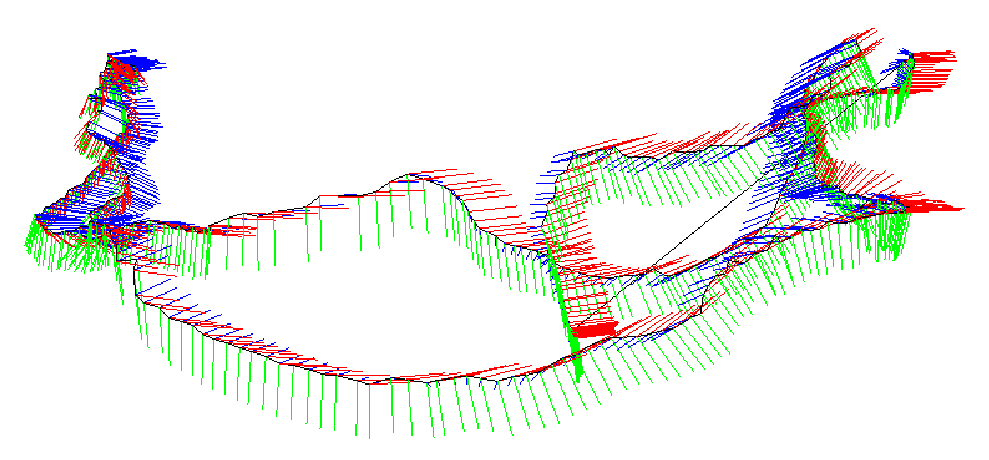
\includegraphics[width=0.8\textwidth]{rigidMotion/trajectory.pdf}
	\caption {Results of pose visualization}
	\label{fig:trajectory}
\end{figure}

\subsection{Displaying Camera Pose}
\begin{figure}[!htp]
	\centering
	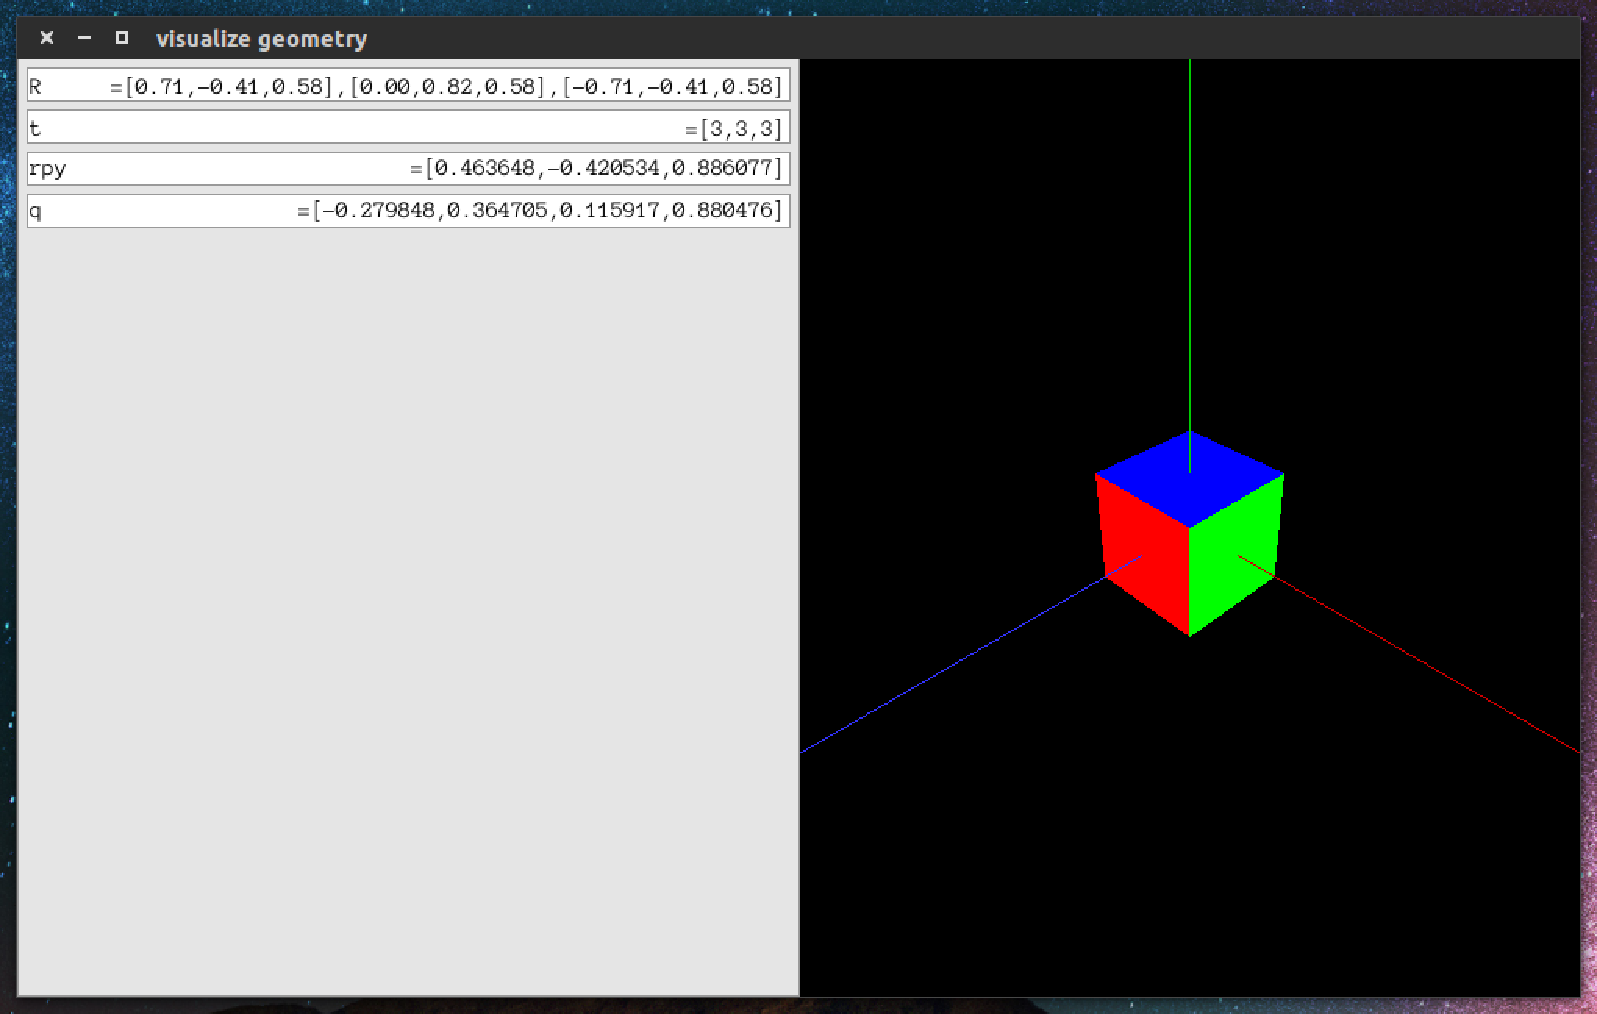
\includegraphics[width=0.8\textwidth]{rigidMotion/visualizeGeometry.pdf}
	\caption {Visualization program for rotation matrix, Euler angle, quaternion. }
	\label{fig:visualizeGeometry}
\end{figure}

In addition to displaying the trajectory, we can also display the camera's pose in the 3D window. In slambook2/ch3/visualizeGeometry, we visualize various expressions of camera poses (see \autoref{fig:visualizeGeometry}). When the reader uses the mouse to move the camera, the box on the left side will display the rotation matrix, translation, Euler angle, and quaternion of the camera pose in real-time. You can see how the data changes. According to our experience, it is hard to infer the exact rotation from quaternions or matrices. However, although the rotation matrix or transformation matrix is not intuitive, it is not difficult to visually display them. This program uses the \textit{Pangolin} library as a 3D display library. Please refer to ``Readme.txt'' to compile the program.

\section*{Exercises}
\begin{enumerate}
	\item Verify that the rotation matrix is an orthogonal matrix.
	\item Prove the Rodrigues formula.
	\item Verify that after the quaternion rotates a point, the result is a imaginary quaternion (the real part is zero), so it still corresponds to a three-dimensional space point, see~\eqref{eq:rotate-with-quaternion}.
	\item Draw a table that summarizes the conversion relationship of the rotation matrix, rotation angle, Euler angle and quaternion.
	\item Suppose there is a large \textit{Eigen} matrix, we want to know the value in the top left $3 \times 3$ blocks, and then assign it to $\mathbf{I}_{3 \times 3}$. Please implement it in C++.
	\item When does a general linear equation $\mathbf{A} \mathbf{x}=\mathbf{b}$ has a unique solution of $\mathbf{x}$? How to solve it numerically? Can you implement it in \textit{Eigen}?
\end{enumerate}
